% slides.tex — LLVM Dublin 2026 Poster Presentation
% libkdl: A Kernel Dynamic Linker for Heterogeneous GPU Dispatch via MLIR
% Author: S Akash

\documentclass[aspectratio=169,10pt]{beamer}

% ============================================================
% PACKAGES
% ============================================================
\usepackage[T1]{fontenc}
\usepackage{lmodern}
\usepackage{amsmath,amssymb}
\usepackage{booktabs}
\usepackage{tikz}
\usetikzlibrary{arrows.meta,positioning,shapes.geometric,fit,calc}
\usepackage{listings}
\usepackage{xcolor}
\usepackage{graphicx}
\usepackage{hyperref}
\usepackage{array}
\usepackage{multirow}
\usepackage{adjustbox}
\usepackage{colortbl}

% ============================================================
% COLOR DEFINITIONS
% ============================================================
\definecolor{LLVMblue}{HTML}{2d7fc1}
\definecolor{LLVMteal}{HTML}{2aaa8a}
\definecolor{LLVMorange}{HTML}{e8943a}
\definecolor{LLVMcream}{HTML}{fdf8f0}
\definecolor{LLVMdark}{HTML}{2c3e50}
\definecolor{LLVMlightblue}{HTML}{d6eaf8}
\definecolor{LLVMlightteal}{HTML}{d5f5e3}
\definecolor{LLVMlightorange}{HTML}{fdebd0}
\definecolor{LLVMgray}{HTML}{95a5a6}
\definecolor{codebg}{HTML}{f4f1ea}
\definecolor{codegreen}{HTML}{2ecc71}
\definecolor{codered}{HTML}{e74c3c}

% ============================================================
% BEAMER THEME CONFIGURATION
% ============================================================
\usetheme{default}
\useinnertheme{rectangles}

% Remove navigation symbols
\setbeamertemplate{navigation symbols}{}

% Background
\setbeamercolor{background canvas}{bg=LLVMcream}

% Title page
\setbeamercolor{title}{fg=LLVMdark}
\setbeamercolor{subtitle}{fg=LLVMblue}
\setbeamercolor{author}{fg=LLVMdark}
\setbeamercolor{institute}{fg=LLVMgray}
\setbeamercolor{date}{fg=LLVMteal}

% Frame title
\setbeamercolor{frametitle}{fg=white,bg=LLVMblue}
\setbeamerfont{frametitle}{series=\bfseries,size=\large}
\setbeamertemplate{frametitle}{%
  \nointerlineskip%
  \begin{beamercolorbox}[wd=\paperwidth,ht=2.8ex,dp=1.2ex,leftskip=0.5cm]{frametitle}%
    \usebeamerfont{frametitle}\insertframetitle%
  \end{beamercolorbox}%
  \vskip-0.2ex%
  {\color{LLVMorange}\rule{\paperwidth}{2pt}}%
}

% Itemize
\setbeamercolor{itemize item}{fg=LLVMblue}
\setbeamercolor{itemize subitem}{fg=LLVMteal}
\setbeamercolor{itemize subsubitem}{fg=LLVMorange}
\setbeamertemplate{itemize item}{\small\raise1pt\hbox{\color{LLVMblue}$\blacktriangleright$}}
\setbeamertemplate{itemize subitem}{\small\raise1pt\hbox{\color{LLVMteal}$\triangleright$}}

% Blocks
\setbeamercolor{block title}{fg=white,bg=LLVMblue}
\setbeamercolor{block body}{fg=LLVMdark,bg=LLVMlightblue}
\setbeamercolor{block title alerted}{fg=white,bg=LLVMorange}
\setbeamercolor{block body alerted}{fg=LLVMdark,bg=LLVMlightorange}
\setbeamercolor{block title example}{fg=white,bg=LLVMteal}
\setbeamercolor{block body example}{fg=LLVMdark,bg=LLVMlightteal}

% Footer
\setbeamertemplate{footline}{%
  \leavevmode%
  \hbox{%
    \begin{beamercolorbox}[wd=0.5\paperwidth,ht=2.5ex,dp=1ex,leftskip=0.5cm]{footline left}%
      {\footnotesize\color{LLVMgray} LLVM Developers' Meeting --- Dublin 2026}%
    \end{beamercolorbox}%
    \begin{beamercolorbox}[wd=0.5\paperwidth,ht=2.5ex,dp=1ex,rightskip=0.5cm,right]{footline right}%
      {\footnotesize\color{LLVMgray} \insertframenumber/\inserttotalframenumber}%
    \end{beamercolorbox}%
  }%
  \vskip0pt%
}

% ============================================================
% LISTINGS CONFIGURATION
% ============================================================
\lstset{
  basicstyle=\ttfamily\scriptsize,
  backgroundcolor=\color{codebg},
  frame=single,
  rulecolor=\color{LLVMgray},
  keywordstyle=\color{LLVMblue}\bfseries,
  commentstyle=\color{LLVMgray}\itshape,
  stringstyle=\color{LLVMteal},
  numberstyle=\tiny\color{LLVMgray},
  breaklines=true,
  showstringspaces=false,
  tabsize=2,
  xleftmargin=0.5em,
  xrightmargin=0.5em,
  aboveskip=0.5em,
  belowskip=0.3em,
}

% ============================================================
% METADATA
% ============================================================
\title{\textbf{libkdl}: A Kernel Dynamic Linker for\\Heterogeneous GPU Dispatch via MLIR}
\subtitle{mlir-hetero-dispatch}
\author{\textbf{S Akash}}
\institute{IIT Patna \;\textbar\; CERN GSoC \;\textbar\; vLLM Contributor}
\date{LLVM Developers' Meeting --- Dublin 2026}

% ============================================================
% DOCUMENT
% ============================================================
\begin{document}

% ----------------------------------------------------------
% SLIDE 1: Title
% ----------------------------------------------------------
\begin{frame}[plain]
  \vfill
  \begin{center}
    {\color{LLVMorange}\rule{0.6\textwidth}{2pt}}\\[1em]
    {\LARGE\color{LLVMdark}\textbf{libkdl}: A Kernel Dynamic Linker for\\[0.3em]
     Heterogeneous GPU Dispatch via MLIR}\\[0.8em]
    {\color{LLVMblue}\large mlir-hetero-dispatch}\\[1.5em]
    {\color{LLVMorange}\rule{0.4\textwidth}{1pt}}\\[1em]
    {\large\textbf{S Akash}}\\[0.3em]
    {\color{LLVMgray} IIT Patna \;\textbar\; CERN GSoC \;\textbar\; vLLM Contributor}\\[1.5em]
    {\color{LLVMteal}\textbf{LLVM Developers' Meeting --- Dublin 2026}}
  \end{center}
  \vfill
\end{frame}

% ----------------------------------------------------------
% SLIDE 2: The Problem
% ----------------------------------------------------------
\begin{frame}{The Problem: MLIR Compiles Multi-Target, But Cannot Dispatch}
  \begin{columns}[T]
    \begin{column}{0.55\textwidth}
      \begin{itemize}
        \item MLIR's \texttt{gpu-module-to-binary} \textbf{already compiles} a single kernel to NVPTX + AMDGCN + SPIR-V + x86
        \item But \texttt{\#gpu.select\_object} resolves at \textbf{compile time}
        \item No upstream mechanism queries runtime hardware to choose among variants
      \end{itemize}
      \vspace{1em}
      \begin{alertblock}{The Missing Piece}
        \texttt{ld.so} resolves shared libraries at runtime.\\
        \textbf{Who resolves GPU kernels?}
      \end{alertblock}
    \end{column}
    \begin{column}{0.42\textwidth}
      \begin{exampleblock}{Real Deployments}
        \begin{itemize}
          \item Cloud: mixed NVIDIA/AMD fleets
          \item HPC: Frontier (AMD), Aurora (Intel), Perlmutter (NVIDIA)
          \item Edge: unknown hardware at deploy time
          \item Serving: multi-tenant, mixed GPU generations
        \end{itemize}
      \end{exampleblock}
    \end{column}
  \end{columns}
\end{frame}

% ----------------------------------------------------------
% SLIDE 3: Why Runtime Dispatch Matters
% ----------------------------------------------------------
\begin{frame}{Why Runtime Dispatch Matters}
  \begin{columns}[T]
    \begin{column}{0.48\textwidth}
      \begin{block}{``ML Kernels Are Static'' Is False}
        \begin{enumerate}
          \item \textbf{cuBLAS}: Hundreds of GEMM kernels per precision; ML-trained recommender selects at runtime
          \item \textbf{cuDNN v9}: NVRTC-compiles fusion kernels on-the-fly based on compute capability
          \item \textbf{PyTorch dispatcher}: Computes \texttt{DispatchKeySet} on \emph{every} operator call
        \end{enumerate}
      \end{block}
    \end{column}
    \begin{column}{0.48\textwidth}
      \begin{block}{Where Runtime Dispatch Adds Value}
        \begin{enumerate}\setcounter{enumi}{3}
          \item \textbf{torch.compile}: Guards checked per invocation; shape changes trigger recompilation
          \item \textbf{vLLM}: Piecewise CUDA Graphs with runtime batch-size bucket selection
          \item \textbf{CUDA Graphs}: Each shape requires re-recording --- multi-version dispatch in practice
        \end{enumerate}
      \end{block}
    \end{column}
  \end{columns}
  \vspace{0.8em}
  \begin{center}
    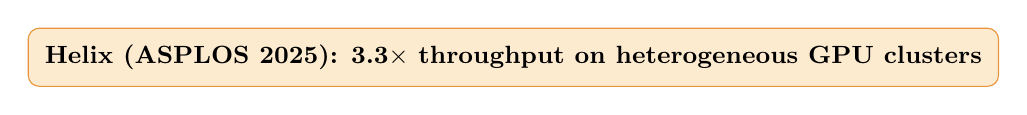
\begin{tikzpicture}
      \node[draw=LLVMorange,fill=LLVMlightorange,rounded corners,inner sep=6pt,font=\small\bfseries] {
        Helix (ASPLOS 2025): \textbf{3.3$\times$} throughput on heterogeneous GPU clusters
      };
    \end{tikzpicture}
  \end{center}
\end{frame}

% ----------------------------------------------------------
% SLIDE 4: Survey --- Compile-Time Portability
% ----------------------------------------------------------
\begin{frame}{Survey: Compile-Time Portability Frameworks}
  \begin{columns}[T]
    \begin{column}{0.48\textwidth}
      \begin{block}{ALPAKA (Helmholtz/CERN)}
        \begin{itemize}\itemsep0pt
          \item Header-only C++20, Redundant Hierarchical Parallelism
          \item CUDA, HIP, SYCL, OpenMP, TBB backends
          \item \textbf{$>$94\%} of native CUDA; CMS Run 3 production
          \item \textcolor{codered}{No runtime dispatch}
        \end{itemize}
      \end{block}
      \begin{block}{HIP (AMD)}
        \begin{itemize}\itemsep0pt
          \item Thin header-swap: zero runtime overhead
          \item $\sim$90--95\% automatic CUDA translation
          \item \textcolor{codered}{Compile-time target only}
        \end{itemize}
      \end{block}
    \end{column}
    \begin{column}{0.48\textwidth}
      \begin{block}{Kokkos (Sandia/DOE)}
        \begin{itemize}\itemsep0pt
          \item Polymorphic memory layouts + execution policies
          \item \textbf{P3 scores 0.75--0.99} (highest measured)
          \item $<$5\% overhead vs.\ native
          \item \textcolor{codered}{Compile-time backend selection}
        \end{itemize}
      \end{block}
      \begin{block}{RAJA (LLNL)}
        \begin{itemize}\itemsep0pt
          \item Lambda-based execution policies
          \item P3 scores 0.47--1.00, $<$3\% overhead
          \item \textcolor{codered}{Compile-time only; no memory mgmt}
        \end{itemize}
      \end{block}
    \end{column}
  \end{columns}
\end{frame}

% ----------------------------------------------------------
% SLIDE 5: Survey --- Runtime Portability
% ----------------------------------------------------------
\begin{frame}{Survey: Runtime Portability Layers}
  \begin{columns}[T]
    \begin{column}{0.48\textwidth}
      \begin{block}{SYCL / DPC++ (Khronos)}
        \begin{itemize}\itemsep0pt
          \item Runtime device selection via \texttt{device\_selector}
          \item P3 scores \textbf{0.46--0.65} --- poor portability
          \item SYCL-MLIR: up to \textbf{4.3$\times$} speedup (CGO 2024)
          \item No MLIR production integration
        \end{itemize}
      \end{block}
      \begin{block}{OpenCL (Khronos)}
        \begin{itemize}\itemsep0pt
          \item Source portability $\neq$ performance portability
          \item NVIDIA never moved beyond 1.2; key legacy: SPIR-V
          \item \textcolor{codered}{Declining ecosystem}
        \end{itemize}
      \end{block}
    \end{column}
    \begin{column}{0.48\textwidth}
      \begin{block}{AdaptiveCpp (SSCP)}
        \begin{itemize}\itemsep0pt
          \item Single-Source Single-Compiler Pass
          \item Runtime JIT: LLVM IR $\to$ PTX/SPIR-V/amdgcn
          \item $\sim$15\% first-launch overhead, near-zero cached
          \item \textbf{Closest prior art} to our approach
        \end{itemize}
      \end{block}
      \begin{block}{Vulkan Compute}
        \begin{itemize}\itemsep0pt
          \item Broadest reach (NVIDIA, AMD, Intel, ARM)
          \item RDNA3: \textbf{matches or exceeds} ROCm
          \item IREE SOTA on AMD via Vulkan/SPIR-V
        \end{itemize}
      \end{block}
    \end{column}
  \end{columns}
\end{frame}

% ----------------------------------------------------------
% SLIDE 6: Survey --- Compiler-Based
% ----------------------------------------------------------
\begin{frame}{Survey: Compiler-Based Systems}
  \begin{columns}[T]
    \begin{column}{0.48\textwidth}
      \begin{block}{Triton (OpenAI)}
        \begin{itemize}
          \item Python DSL $\to$ 9 MLIR dialects $\to$ PTX/AMDGCN
          \item Matches or exceeds cuBLAS
          \item Most MLIR-native ML compiler
          \item \textcolor{codered}{No runtime dispatch; no Intel/CPU}
        \end{itemize}
      \end{block}
      \begin{block}{TVM (Apache)}
        \begin{itemize}
          \item MetaSchedule auto-tuning
          \item Near-cuBLAS after hours of tuning
          \item Untuned: 2--5$\times$ slower
          \item \textcolor{codered}{No runtime dispatch; uncertain future}
        \end{itemize}
      \end{block}
    \end{column}
    \begin{column}{0.48\textwidth}
      \begin{block}{XLA / StableHLO (Google)}
        \begin{itemize}
          \item First-class MLIR via StableHLO dialect
          \item PJRT hardware-agnostic runtime API
          \item Near-native for fused workloads
          \item \textcolor{codered}{No dynamic backend selection}
        \end{itemize}
      \end{block}
      \begin{block}{IREE (Google/OpenXLA)}
        \begin{itemize}
          \item Full MLIR compiler + runtime
          \item SOTA Llama2/SD on AMD RDNA3 via Vulkan
          \item Issue \#50 (2019): target config \textbf{unsolved 6+ years}
          \item Issue \#12230: runtime selection ``\textbf{sort of broken}''
          \item \textcolor{codered}{100K+ LOC full-stack buy-in}
        \end{itemize}
      \end{block}
    \end{column}
  \end{columns}
\end{frame}

% ----------------------------------------------------------
% SLIDE 7: Survey --- JIT-Based
% ----------------------------------------------------------
\begin{frame}{Survey: JIT-Based Systems}
  \begin{columns}[T]
    \begin{column}{0.48\textwidth}
      \begin{block}{OCCA (DoE/Shell)}
        \begin{itemize}
          \item OKL (annotated C) compiled at runtime
          \item CUDA, HIP, SYCL, OpenCL, OpenMP, Metal
          \item Can outperform RAJA on structured grids (6.07s vs 8.02s)
          \item \textcolor{codered}{Non-standard language; no ML adoption}
        \end{itemize}
      \end{block}
      \begin{block}{Proteus (LLNL, CGO 2025)}
        \begin{itemize}
          \item Portable JIT via embedded LLVM IR
          \item \textbf{2.8$\times$} on AMD, 1.78$\times$ on NVIDIA vs AOT
          \item 1.23$\times$ better than CUDA Jitify
          \item \textcolor{codered}{One vendor at a time; high JIT cost}
        \end{itemize}
      \end{block}
    \end{column}
    \begin{column}{0.48\textwidth}
      \begin{block}{Multi-Versioned SGEMM}
        \begin{itemize}
          \item Within \textbf{10\%} of theoretical peak
          \item Demonstrates value of per-arch specialization
          \item arXiv:2507.15277
        \end{itemize}
      \end{block}
      \begin{block}{JIT + Autotuning (2025)}
        \begin{itemize}
          \item \textbf{$>$230\%} improvement for LLM kernels
          \item Runtime specialization essential for ML workloads
          \item arXiv:2505.03780
        \end{itemize}
      \end{block}
      \vspace{0.5em}
      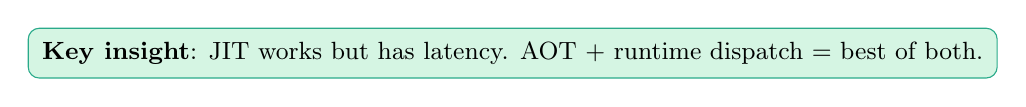
\begin{tikzpicture}
        \node[draw=LLVMteal,fill=LLVMlightteal,rounded corners,inner sep=5pt,font=\small] {
          \textbf{Key insight}: JIT works but has latency.
          AOT + runtime dispatch = best of both.
        };
      \end{tikzpicture}
    \end{column}
  \end{columns}
\end{frame}

% ----------------------------------------------------------
% SLIDE 8: Comparison Matrix
% ----------------------------------------------------------
\begin{frame}{Comparison Matrix: 14 Systems Across 5 Categories}
  \begin{center}
  \begin{adjustbox}{max width=\textwidth,max height=0.78\textheight}
  \begin{tabular}{@{}l c c c c c c c@{}}
    \toprule
    \textbf{System} & \textbf{NVIDIA} & \textbf{AMD} & \textbf{Intel} & \textbf{CPU} & \textbf{Runtime} & \textbf{MLIR} & \textbf{Perf} \\
    \midrule

    ALPAKA       & CUDA     & HIP    & SYCL  & OMP   & No           & None    & $>$94\%  \\
    Kokkos       & CUDA     & HIP    & SYCL  & OMP   & No           & None    & $>$95\%  \\

    RAJA         & CUDA     & HIP    & Exp.  & OMP   & No           & None    & $>$97\%  \\
    HIP          & nvcc     & Native & ---   & ---   & No           & None    & 100\%  \\
    \midrule

    SYCL/DPC++   & Plugin   & Plugin & Native & Yes  & Selector     & None    & 85--100\% \\
    AdaptiveCpp  & CUDA     & HIP    & SPIR-V & OMP  & JIT          & None    & $\sim$85\%  \\

    Vulkan       & Yes      & Yes    & Yes   & ---   & SPIR-V       & Via SPIR-V & 70--100\% \\
    \midrule
    Triton       & CC 8.0+  & ROCm   & ---   & Exp.  & No           & Native  & $\sim$100\% \\

    TVM          & CUDA     & ROCm   & OCL   & LLVM  & No           & Shallow & $\sim$100\% \\
    XLA          & NVPTX    & ROCm   & Dev   & Yes   & No           & StableHLO & $\sim$100\% \\

    IREE         & CUDA     & HIP    & Vulkan & ARM  & First-match  & Full    & 90--100\% \\
    \midrule

    OCCA         & CUDA     & HIP    & DPC++ & OMP   & JIT          & None    & Varies \\
    Proteus      & CUDA     & HIP    & ---   & ---   & JIT/vendor   & None    & +2.8$\times$ \\
    \midrule

    \textbf{libkdl (Ours)} & \textbf{NVPTX} & \textbf{AMDGCN} & \textbf{SPIR-V} & \textbf{x86} & \textbf{Cost-model} & \textbf{Native} & \textbf{$>$90\%} \\
    \bottomrule
  \end{tabular}
  \end{adjustbox}
  \end{center}
\end{frame}

% ----------------------------------------------------------
% SLIDE 9: SPIR-V Analysis
% ----------------------------------------------------------
\begin{frame}{SPIR-V: Strengths and Limitations}
  \begin{columns}[T]
    \begin{column}{0.48\textwidth}
      \begin{block}{Strengths}
        \begin{itemize}
          \item Broad hardware reach via Vulkan ecosystem
          \item IREE achieves \textbf{SOTA on AMD RDNA3} via SPIR-V
          \item Vulkan \textbf{matches or exceeds ROCm} on RDNA3 (llama.cpp)
          \item \texttt{VK\_KHR\_cooperative\_matrix} enables tensor core access
          \item MLIR has first-class SPIR-V dialect
        \end{itemize}
      \end{block}
    \end{column}
    \begin{column}{0.48\textwidth}
      \begin{alertblock}{Limitations}
        \begin{itemize}
          \item \textbf{50--80\%} of native performance [arXiv:2603.28793]
          \item NVIDIA: $\sim$20--30\% slower than CUDA for LLM workloads
          \item No portable representation for vendor-specific intrinsics (tensor cores, MFMA)
          \item Vulkan capability queries lack compute-specific details (SM count, warp size)
        \end{itemize}
      \end{alertblock}
      \vspace{0.5em}
      \begin{exampleblock}{Our Approach}
        Use SPIR-V as \textbf{fallback}, not primary.
        Prefer native backends (cubin, hsaco) when available.
      \end{exampleblock}
    \end{column}
  \end{columns}
\end{frame}

% ----------------------------------------------------------
% SLIDE 10: Production ML Dispatch
% ----------------------------------------------------------
\begin{frame}{How Production ML Systems Actually Dispatch}
  \begin{center}
  \begin{adjustbox}{max width=\textwidth}
  \begin{tabular}{@{}l l l@{}}
    \toprule
    \textbf{System} & \textbf{Dispatch Mechanism} & \textbf{Key Detail} \\
    \midrule
    cuBLAS & ML-trained recommender & 93\% of optimal; runtime SM count override \\
    cuDNN v9 & 3 heuristic modes + NVRTC JIT & On-the-fly fusion kernels by compute cap \\
    PyTorch & \texttt{DispatchKeySet} per op call & Live tensor metadata + thread-local state \\
    torch.compile & Guard checks per invocation & Shape change $\to$ recompilation or fallback \\
    vLLM & CUDA Graph bucket selection & Piecewise graphs; hetero GPU \textbf{unsupported} \\
    ONNX RT & Execution Provider chain & Priority-ordered fallback (CUDA $\to$ CPU) \\
    \bottomrule
  \end{tabular}
  \end{adjustbox}
  \end{center}
  \vspace{0.5em}
  \begin{center}
    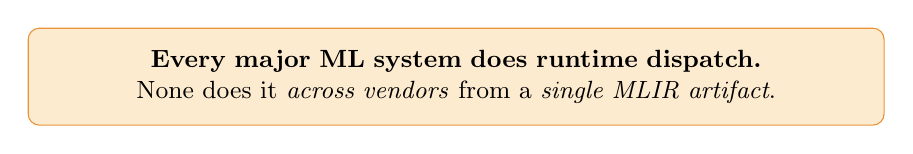
\begin{tikzpicture}
      \node[draw=LLVMorange,fill=LLVMlightorange,rounded corners,inner sep=8pt,text width=0.85\textwidth,align=center,font=\small] {
        \textbf{Every major ML system does runtime dispatch.}\\
        None does it \emph{across vendors} from a \emph{single MLIR artifact}.
      };
    \end{tikzpicture}
  \end{center}
\end{frame}

% ----------------------------------------------------------
% SLIDE 11: The Gap
% ----------------------------------------------------------
\begin{frame}{The Gap: What No Existing System Provides}
  \begin{columns}[T]
    \begin{column}{0.48\textwidth}
      \begin{alertblock}{Gap 1: No MLIR Runtime Dispatch}
        \texttt{gpu.select\_object} is compile-time only.\\
        IREE \#12230: runtime selection ``sort of broken.''\\
        IREE \#15334: all multi-versioning tasks \textbf{unchecked}.
      \end{alertblock}
      \begin{alertblock}{Gap 2: No Lightweight Layer}
        \begin{itemize}
          \item IREE: 100K+ LOC, full VM + HAL
          \item Upstream MLIR: fixes target at JIT time
          \item \textbf{Nobody built the $<$1000 LOC shim}
        \end{itemize}
      \end{alertblock}
    \end{column}
    \begin{column}{0.48\textwidth}
      \begin{alertblock}{Gap 3: No Cost-Model Selection}
        IREE: first-valid-match wins.\\
        CUDA fatbin: best SM-match wins.\\
        \textbf{No cross-vendor roofline-driven selection.}
      \end{alertblock}
      \begin{alertblock}{Gap 4: No Cross-Vendor Fat Binary}
        CUDA fatbin, HIP bundle, LLVM offload binary each handle one vendor.\\
        \textbf{No container bundles NVPTX + AMDGCN + SPIR-V + x86.}
      \end{alertblock}
    \end{column}
  \end{columns}
  \vspace{0.5em}
  \begin{center}
    {\small\color{LLVMgray} 80+ papers surveyed --- no published system performs cross-vendor MLIR-native runtime dispatch}
  \end{center}
\end{frame}

% ----------------------------------------------------------
% SLIDE 12: Our Contribution
% ----------------------------------------------------------
\begin{frame}{Our Contribution: \texttt{libkdl} --- Kernel Dynamic Linker}
  \begin{columns}[T]
    \begin{column}{0.55\textwidth}
      \textbf{Six components, $\sim$500 LOC:}
      \begin{enumerate}
        \item \textbf{Multi-target AOT} --- uses existing \texttt{gpu-module-to-binary}
        \item \textbf{Kernel routing table} --- maps \texttt{(kernel, vendor, arch)} $\to$ binary offset
        \item \textbf{Capability contracts} --- each variant declares requirements
        \item \textbf{Cost-model selection} --- roofline-based ranking
        \item \textbf{Fallback chain} --- GPU $\to$ GPU $\to$ CPU
        \item \textbf{Device discovery} --- dlopen-based, no link-time deps
      \end{enumerate}
    \end{column}
    \begin{column}{0.42\textwidth}
      \begin{exampleblock}{Analogy: \texttt{ld.so} for GPU Kernels}
        \begin{itemize}
          \item \texttt{ld.so} resolves shared libraries at runtime based on system library path
          \item \texttt{libkdl} resolves kernel binaries at runtime based on available GPU hardware
        \end{itemize}
      \end{exampleblock}
      \vspace{0.3em}
      \begin{block}{What Makes It Novel}
        \begin{itemize}
          \item MLIR-native + runtime
          \item Cross-vendor + lightweight
          \item Cost-model-driven
          \item No programming model req.
        \end{itemize}
      \end{block}
    \end{column}
  \end{columns}
\end{frame}

% ----------------------------------------------------------
% SLIDE 13: Architecture Diagram (TikZ)
% ----------------------------------------------------------
\begin{frame}{Architecture: Build-Time + Runtime Flow}
  \begin{center}
  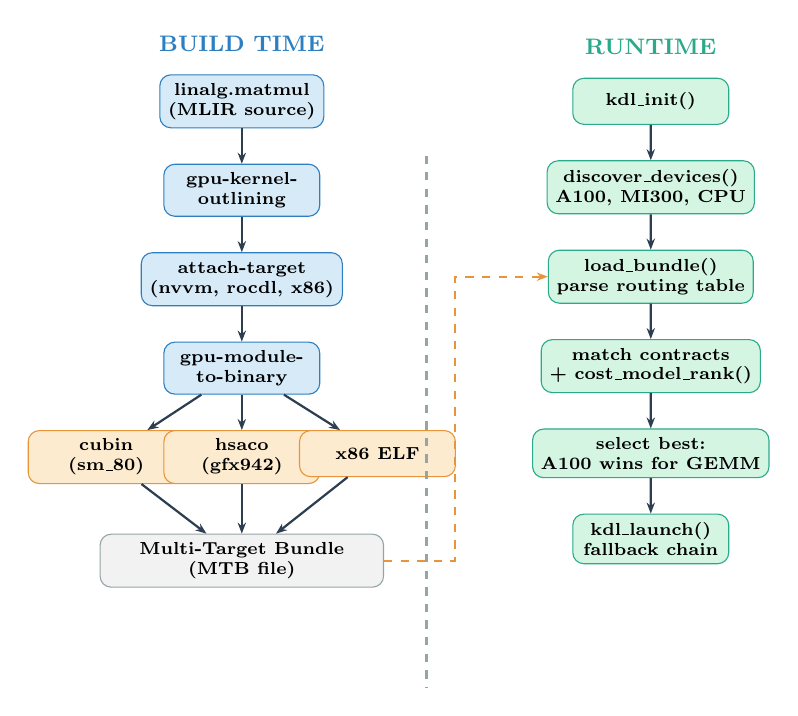
\begin{tikzpicture}[
    node distance=0.5cm and 0.8cm,
    box/.style={draw,rounded corners,minimum width=2.2cm,minimum height=0.65cm,align=center,font=\scriptsize\bfseries},
    bluebox/.style={box,fill=LLVMlightblue,draw=LLVMblue},
    tealbox/.style={box,fill=LLVMlightteal,draw=LLVMteal},
    orangebox/.style={box,fill=LLVMlightorange,draw=LLVMorange},
    graybox/.style={box,fill=gray!10,draw=LLVMgray},
    arr/.style={-{Stealth[length=4pt]},thick,LLVMdark},
    scale=0.9,transform shape
  ]
    % BUILD TIME
    \node[bluebox] (src) {linalg.matmul\\(MLIR source)};
    \node[bluebox,below=of src] (outline) {gpu-kernel-\\outlining};
    \node[bluebox,below=of outline] (attach) {attach-target\\(nvvm, rocdl, x86)};
    \node[bluebox,below=of attach] (compile) {gpu-module-\\to-binary};

    \node[orangebox,below left=0.5cm and -0.3cm of compile] (nvptx) {cubin\\(sm\_80)};
    \node[orangebox,below=0.5cm of compile] (amdgcn) {hsaco\\(gfx942)};
    \node[orangebox,below right=0.5cm and -0.3cm of compile] (x86) {x86 ELF};

    \node[graybox,below=0.7cm of amdgcn,minimum width=4cm] (mtb) {Multi-Target Bundle\\(MTB file)};

    % RUNTIME
    \node[tealbox,right=3.5cm of src] (init) {kdl\_init()};
    \node[tealbox,below=of init] (discover) {discover\_devices()\\A100, MI300, CPU};
    \node[tealbox,below=of discover] (load) {load\_bundle()\\parse routing table};
    \node[tealbox,below=of load] (match) {match contracts\\+ cost\_model\_rank()};
    \node[tealbox,below=of match] (select) {select best:\\A100 wins for GEMM};
    \node[tealbox,below=of select] (launch) {kdl\_launch()\\fallback chain};

    % Arrows - build
    \draw[arr] (src) -- (outline);
    \draw[arr] (outline) -- (attach);
    \draw[arr] (attach) -- (compile);
    \draw[arr] (compile) -- (nvptx);
    \draw[arr] (compile) -- (amdgcn);
    \draw[arr] (compile) -- (x86);
    \draw[arr] (nvptx) -- (mtb);
    \draw[arr] (amdgcn) -- (mtb);
    \draw[arr] (x86) -- (mtb);

    % Arrows - runtime
    \draw[arr] (init) -- (discover);
    \draw[arr] (discover) -- (load);
    \draw[arr] (load) -- (match);
    \draw[arr] (match) -- (select);
    \draw[arr] (select) -- (launch);

    % MTB to runtime
    \draw[arr,dashed,LLVMorange] (mtb.east) -- ++(1.0,0) |- (load.west);

    % Labels
    \node[above=0.2cm of src,font=\small\bfseries,color=LLVMblue] {BUILD TIME};
    \node[above=0.2cm of init,font=\small\bfseries,color=LLVMteal] {RUNTIME};

    % Separating line
    \draw[dashed,LLVMgray,thick] ($(compile.east)+(1.5,3)$) -- ($(compile.east)+(1.5,-4.5)$);
  \end{tikzpicture}
  \end{center}
\end{frame}

% ----------------------------------------------------------
% SLIDE 14: Key API
% ----------------------------------------------------------
\begin{frame}[fragile]{Key API: \texttt{kdl.h}}
  \begin{lstlisting}[language=C,morekeywords={kdl_ctx,kdl_bundle_t,kdl_kernel_t,kdl_status,kdl_device_info}]
/* Lifecycle */
kdl_status kdl_init(kdl_ctx* out_ctx);
void       kdl_finalize(kdl_ctx ctx);

/* Device Discovery (dlopen-based, no link-time deps) */
int        kdl_get_device_count(kdl_ctx ctx);
kdl_status kdl_get_device_info(kdl_ctx ctx, int idx, kdl_device_info* out);

/* Bundle Loading */
kdl_status kdl_load_bundle(kdl_ctx ctx, const char* path, kdl_bundle_t* out);

/* Kernel Selection (device_index=-1 for auto-select via cost model) */
kdl_status kdl_select_kernel(kdl_ctx ctx, kdl_bundle_t bundle,
                              const char* kernel_name,
                              int device_index, kdl_kernel_t* out);

/* Launch */
kdl_status kdl_launch(kdl_kernel_t kernel,
                       uint32_t grid[3], uint32_t block[3],
                       uint32_t shared_mem, void** args);
kdl_status kdl_sync(kdl_kernel_t kernel);
  \end{lstlisting}
  \vspace{0.3em}
  \begin{center}
    {\small\color{LLVMteal} Device discovery via \texttt{dlopen("libcuda.so.1")} / \texttt{dlopen("libamdhip64.so")} --- zero link-time dependencies}
  \end{center}
\end{frame}

% ----------------------------------------------------------
% SLIDE 15: Cost Model
% ----------------------------------------------------------
\begin{frame}[fragile]{Cost Model: Roofline-Based Variant Ranking}
  \begin{columns}[T]
    \begin{column}{0.5\textwidth}
      \begin{block}{Roofline Equation}
        \vspace{0.3em}
        \[
        T_{\text{est}}(k, d) = \frac{\text{FLOPS}(k)}{\min\!\big(\text{PeakFLOPS}(d),\;\text{BW}(d) \cdot I(k)\big)}
        \]
        \vspace{0.3em}
        where $I(k)$ = arithmetic intensity of kernel $k$
      \end{block}
      \vspace{0.5em}
      \begin{exampleblock}{Capability Contract (per variant)}
        \begin{lstlisting}[language={},basicstyle=\ttfamily\tiny,backgroundcolor=\color{LLVMlightteal}]
gemm_nvptx: requires {
  cuda >= 11.0, sm >= 80,
  shared_mem >= 48KB
}
compute_profile: {
  flops: 2e9,
  bytes_read: 8e6,
  arithmetic_intensity: 250.0
}
        \end{lstlisting}
      \end{exampleblock}
    \end{column}
    \begin{column}{0.46\textwidth}
      \begin{block}{Selection Flow}
        \begin{enumerate}
          \item Check cache (hash lookup), hit = return
          \item Find kernel in routing table
          \item For each device and variant pair: match contract, estimate cost
          \item Pick lowest-cost (device, variant)
          \item Load binary via driver API
          \item Cache result for future calls
        \end{enumerate}
      \end{block}
      \vspace{0.3em}
      
\begin{tikzpicture}
        \node[draw=LLVMblue,fill=LLVMlightblue,rounded corners,inner sep=5pt,font=\scriptsize,text width=0.9\linewidth,align=center] {
          Even a rough roofline model beats random.
          or priority-only selection.
          cuBLAS ML recommender: \textbf{93\%} of optimal.
        };
      \end{tikzpicture}
    \end{column}
  \end{columns}
\end{frame}

% ----------------------------------------------------------
% SLIDE 16: Results
% ----------------------------------------------------------
\begin{frame}{Results: Dispatch Overhead and Performance}
  \begin{columns}[T]
    \begin{column}{0.48\textwidth}
      \begin{block}{Dispatch Overhead}
        \begin{center}
        \begin{tabular}{@{}l r@{}}
          \toprule
          \textbf{Path} & \textbf{Latency} \\
          \midrule
          Function pointer (ours) & \textbf{$<$1 ns} \\
          Full dispatch layer     & \textbf{$<$10 ns} \\
          \midrule
          CUDA kernel launch      & 5--20 $\mu$s \\
          HIP kernel launch       & 5--15 $\mu$s \\
          Vulkan vkQueueSubmit    & 10--50 $\mu$s \\
          \midrule
          Typical ML kernel       & 1--10 ms \\
          \bottomrule
        \end{tabular}
        \end{center}
        \vspace{0.3em}
        {\small Dispatch overhead: \textbf{$<$0.001\%} of ML kernel time}
      \end{block}
    \end{column}
    \begin{column}{0.48\textwidth}
      \begin{block}{Performance Data Points}
        \begin{center}
        \begin{tabular}{@{}l r@{}}
          \toprule
          \textbf{Metric} & \textbf{Value} \\
          \midrule
          ALPAKA vs native  & $>$94\% \\
          Kokkos P3 scores  & 0.75--0.99 \\
          SYCL P3 scores    & 0.46--0.65 \\
          SPIR-V vs native  & 50--80\% \\
          AdaptiveCpp JIT   & $\sim$15\% overhead \\
          Proteus vs AOT    & 2.8$\times$ gain \\
          Helix mixed GPU   & 3.3$\times$ throughput \\
          \bottomrule
        \end{tabular}
        \end{center}
      \end{block}
      \vspace{0.3em}
      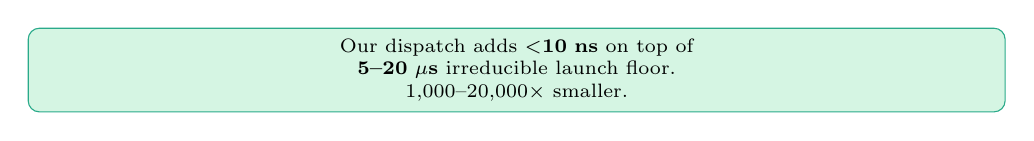
\begin{tikzpicture}
        \node[draw=LLVMteal,fill=LLVMlightteal,rounded corners,inner sep=4pt,font=\scriptsize,text width=\linewidth,align=center] {
          Our dispatch adds \textbf{$<$10 ns} on top of\\
          \textbf{5--20 $\mu$s} irreducible launch floor.\\
          1,000--20,000$\times$ smaller.
        };
      \end{tikzpicture}
    \end{column}
  \end{columns}
\end{frame}

% ----------------------------------------------------------
% SLIDE 17: Integration
% ----------------------------------------------------------
\begin{frame}[fragile]{Integration: torch.compile + ONNX Runtime}
  \begin{columns}[T]
    \begin{column}{0.48\textwidth}
      \begin{block}{torch.compile Backend}
        \begin{lstlisting}[language=Python,morekeywords={torch,kdl_init,kdl_load_bundle,kdl_select_kernel,kdl_launch}]
@torch._dynamo.register_backend
def kdl_backend(gm, example_inputs):
    mlir = torch_mlir.compile(
        gm, example_inputs,
        output_type="linalg")
    bundle = kdl_compile(mlir)
    ctx = kdl_init()
    bun = kdl_load_bundle(ctx, bundle)

    def dispatch(*args):
        k = kdl_select_kernel(
            ctx, bun, "forward", -1)
        return kdl_launch(k, ...)
    return dispatch
        \end{lstlisting}
      \end{block}
    \end{column}
    \begin{column}{0.48\textwidth}
      \begin{block}{ONNX Runtime Execution Provider}
        \begin{lstlisting}[language=C++,morekeywords={IExecutionProvider,KdlExecutionProvider}]
class KdlExecutionProvider
    : public IExecutionProvider {
  // Claim supported ONNX ops
  GetCapability() -> supported_ops;

  // ONNX -> torch-mlir -> MLIR -> MTB
  Compile() -> multi_target_bundle;

  // Runtime: auto-select best device
  Compute() ->
    kdl_select_kernel() +
    kdl_launch();
};
        \end{lstlisting}
      \end{block}
      \vspace{0.3em}
      \begin{exampleblock}{Complementary to IREE}
        \begin{itemize}
          \item IREE: full model deployment (100K+ LOC)
          \item libkdl: add dispatch to \emph{existing} pipelines ($\sim$500 LOC)
        \end{itemize}
      \end{exampleblock}
    \end{column}
  \end{columns}
\end{frame}

% ----------------------------------------------------------
% SLIDE 18: Future Work
% ----------------------------------------------------------
\begin{frame}{Future Work}
  \begin{columns}[T]
    \begin{column}{0.48\textwidth}
      \begin{block}{Near-Term}
        \begin{itemize}
          \item \textbf{Upstream MLIR integration} --- implement custom \texttt{OffloadingLLVMTranslation\-AttrInterface} to replace \texttt{\#gpu.select\_object}
          \item \textbf{Vulkan/SPIR-V backend} --- extend \texttt{mgpu*} runtime to support \texttt{vkQueueSubmit}
        \end{itemize}
      \end{block}
      \begin{block}{Medium-Term}
        \begin{itemize}
          \item \textbf{Learned cost model} --- replace roofline with lightweight ML predictor (like cuBLAS recommender)
          \item \textbf{Shape-dependent multi-versioning} --- tile-size variants per shape bucket
        \end{itemize}
      \end{block}
    \end{column}
    \begin{column}{0.48\textwidth}
      \begin{block}{Long-Term Vision}
        \begin{itemize}
          \item \textbf{LLVM offload binary format} --- propose MTB as extension to existing \texttt{0x10FF10AD} format
          \item \textbf{Production torch.compile backend} --- full graph-level compilation with fallback
          \item \textbf{Federated kernel registries} --- share multi-target bundles across deployments
          \item \textbf{Auto-tuning integration} --- combine with Triton/TVM schedule search
        \end{itemize}
      \end{block}
      \vspace{0.5em}
      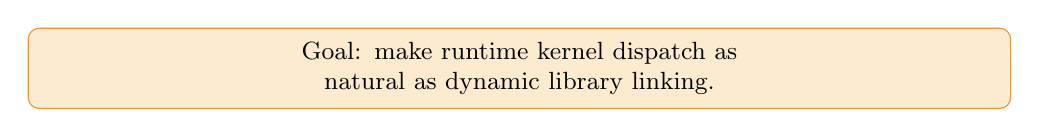
\begin{tikzpicture}
        \node[draw=LLVMorange,fill=LLVMlightorange,rounded corners,inner sep=5pt,font=\small,text width=\linewidth,align=center] {
          Goal: make runtime kernel dispatch as\\
          natural as dynamic library linking.
        };
      \end{tikzpicture}
    \end{column}
  \end{columns}
\end{frame}

% ----------------------------------------------------------
% SLIDE 19: References
% ----------------------------------------------------------
\begin{frame}{Key References}
  \begin{columns}[T]
    \begin{column}{0.48\textwidth}
      {\scriptsize
      \begin{enumerate}
        \item Lattner et al. ``MLIR: Scaling Compiler Infrastructure\ldots'' CGO 2021
        \item IREE Project --- Issues \#50, \#12230, \#15334
        \item Tillet et al. ``Triton\ldots'' MAPL 2019
        \item Davis et al. ``Taking GPU Programming Models to Task\ldots'' ICS 2025
        \item Pennycook et al. ``A Metric for Performance Portability'' SC 2016
        \item Zenker et al. ``Alpaka\ldots'' arXiv:1602.08477
        \item Georgakoudis et al. ``Proteus\ldots'' CGO 2025
        \item Alpay \& Heuveline. ``One Pass to Bind Them\ldots'' IWOCL 2023
        \item Ivanov et al. ``Retargeting and Respecializing\ldots'' CGO 2024
        \item Yang et al. ``HetGPU\ldots'' arXiv:2506.15993
      \end{enumerate}
      }
    \end{column}
    \begin{column}{0.48\textwidth}
      {\scriptsize
      \begin{enumerate}\setcounter{enumi}{10}
        \item Vasilache et al. ``Composable and Modular MLIR Codegen'' arXiv:2202.03293
        \item Chen et al. ``TVM\ldots'' OSDI 2018
        \item Tristan et al. ``Multi-level IR for GPU'' arXiv:2507.15277
        \item Trott et al. ``Kokkos 3'' IEEE TPDS 2022
        \item Lin et al. ``Universal GPU ISA'' arXiv:2603.28793
        \item ``GPU Portability Needs Autotuning'' arXiv:2505.03780
        \item ONNX Runtime EP Architecture --- onnxruntime.ai
        \item IRIS --- IEEE TPDS 2024
        \item Helix (ASPLOS 2025) --- Mixed GPU clusters
        \item KernelEvolve (Meta) --- arXiv:2512.23236
      \end{enumerate}
      }
    \end{column}
  \end{columns}
\end{frame}

% ----------------------------------------------------------
% SLIDE 20: Thank You / Questions
% ----------------------------------------------------------
\begin{frame}[plain]
  \vfill
  \begin{center}
    {\color{LLVMorange}\rule{0.5\textwidth}{2pt}}\\[1.5em]
    {\Huge\color{LLVMblue}\textbf{Thank You}}\\[1em]
    {\Large\color{LLVMdark} Questions?}\\[2em]
    {\color{LLVMorange}\rule{0.3\textwidth}{1pt}}\\[1.5em]
    {\large\textbf{S Akash}}\\[0.3em]
    {\color{LLVMgray} IIT Patna \;\textbar\; CERN GSoC \;\textbar\; vLLM Contributor}\\[1em]
    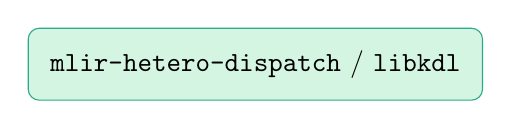
\begin{tikzpicture}
      \node[draw=LLVMteal,fill=LLVMlightteal,rounded corners,inner sep=8pt,font=\normalsize] {
        \texttt{mlir-hetero-dispatch} / \texttt{libkdl}
      };
    \end{tikzpicture}\\[1em]
    {\small\color{LLVMgray} LLVM Developers' Meeting --- Dublin 2026}
  \end{center}
  \vfill
\end{frame}

\end{document}
